% - Pontos A(0,0), B(0,3), C(5,3), D(5,0)
% - Apoio móvel em A, apoio fixo em D
% - Carga de 10kN aplicada entre A e B (ponto médio M em 0, 1.5)
% - Carga distribuída de 6kN/m entre B e C

\documentclass[tikz]{standalone}
\usepackage{stanli}
\usetikzlibrary{calc}

\begin{document}
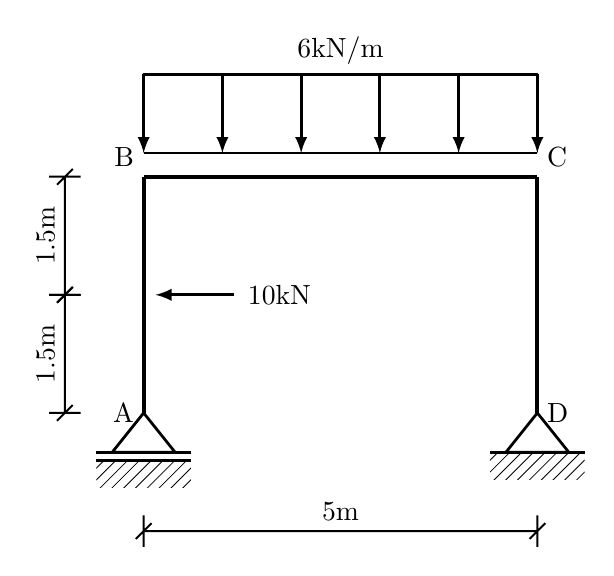
\begin{tikzpicture}
    % Definição dos pontos principais
    \point{A}{0}{0}
    \point{B}{0}{3}
    \point{C}{5}{3}
    \point{D}{5}{0}
    
    % Ponto médio para a carga pontual de 10kN
    \point{M}{0}{1.5}

    % Definição dos apoios
    \support{2}{A} % Apoio móvel
    \support{1}{D} % Apoio fixo

    % Definição das barras (pórtico)
    \beam{2}{A}{B}
    \beam{2}{B}{C}
    \beam{2}{C}{D}

    % Cargas
    % Carga pontual de 10kN no meio da barra AB (sentido horizontal para a direita)
    \load{1}{M}[0] 
    
    % Carga distribuída de 6kN/m na barra BC
    \lineload{1}{B}{C}

    % Notações e Etiquetas
    \notation{1}{A}{A}[left]
    \notation{1}{B}{B}[above left]
    \notation{1}{C}{C}[above right]
    \notation{1}{D}{D}[right]
    
    \notation{1}{M}{10kN}[right=12mm]
        \notation{5}{B}{C}[6kN/m][.5][above=13mm]

    \dimensioning{2}{A}{M}{-10mm}[1.5m]
    \dimensioning{2}{M}{B}{-10mm}[1.5m]
    \dimensioning{1}{B}{C}{-15mm}[5m]
\end{tikzpicture}
\end{document}